%%

%\section*{\MakeUppercase{Загальна характеристика роботи}}
%\section*{\MakeUppercase{
%\textcolor{white}{[1--25]}
%Загальна характеристика роботи
%\textcolor{white}
%{\cite{Olikh2018JAP,Olikh2018SM,Olikh:Ultras2016,Olikh2016JSem,
%Olikh:Rev,OlikhJAP,Olikh:Ultras,Olikh:UPJ2014,
%Olikh:2013IEEE,Olikh:SEMT2013,Olikh:FTP2013,Olikh:UPJ2013,
%Olikh:FTP2011,Olikh:SEMT2011,Olikh:UPJ2010,Gorb2010,Olikh:FTP2009,
%Olikh:SEMT2007,Olikh:MRS2007,Olikh:PZTF2006,
%Olikh:PhChOM2005,Olikh:PJE2004,Olikh:SEMT2004,Olikh:SPQEO2003,
%Olikh:Visn2003,
%1UNCPS,3Tomsk,1SEMST,50IUFFC,9APTTE,2005IUS,ICU2007SC,ICU2007GA,2007MRS,3UNCPS,6DrogGorb,6Drog,
%4UNCPS,4Kremen,7Drog,5UNCPS,2012Ternop,14Plivk,8Drog,2013Buk,6UNCPS,2014IUSOl,2014IUS,6SEMST,
%2015ICU,6CPFCS,7UNCPS,2017MEICS}}}}
%\end{center}%

\begin{center}
\section*{
\textcolor{white}{[1--25]}
\MakeUppercase{Загальна характеристика роботи}
\textcolor{white}
{\cite{Olikh2018JAP,Olikh2018SM,Olikh:Ultras2016,Olikh2016JSem,
Olikh:Rev,OlikhJAP,Olikh:Ultras,Olikh:UPJ2014,
Olikh:2013IEEE,Olikh:SEMT2013,Olikh:FTP2013,Olikh:UPJ2013,
Olikh:FTP2011,Olikh:SEMT2011,Olikh:UPJ2010,Gorb2010,Olikh:FTP2009,
Olikh:SEMT2007,Olikh:MRS2007,Olikh:PZTF2006,
Olikh:PhChOM2005,Olikh:PJE2004,Olikh:SEMT2004,Olikh:SPQEO2003,
Olikh:Visn2003,
1UNCPS,3Tomsk,1SEMST,50IUFFC,9APTTE,2005IUS,ICU2007SC,ICU2007GA,2007MRS,3UNCPS,6DrogGorb,6Drog,
4UNCPS,4Kremen,7Drog,5UNCPS,2012Ternop,14Plivk,8Drog,2013Buk,6UNCPS,2014IUSOl,2014IUS,6SEMST,
2015ICU,6CPFCS,7UNCPS,2017MEICS}}
}
\end{center}




%{\actuality} Обзор, введение в тему, обозначение места данной работы в
%мировых исследованиях и~т.\:п., можно использовать ссылки на~другие
%работы\ifnumequal{\value{bibliosel}}{1}{~\autocite{Gosele1999161}}{}
%(если их~нет, то~в~автореферате
%автоматически пропадёт раздел <<Список литературы>>). Внимание! Ссылки
%на~другие работы в разделе общей характеристики работы можно
%использовать только при использовании \verb!biblatex! (из-за технических
%ограничений \verb!bibtex8!. Это связано с тем, что одна
%и~та~же~характеристика используются и~в~тексте диссертации, и в
%автореферате. В~последнем, согласно ГОСТ, должен присутствовать список
%работ автора по~теме диссертации, а~\verb!bibtex8! не~умеет выводить в одном
%файле два списка литературы).
%При использовании \verb!biblatex! возможно использование исключительно
%в~автореферате подстрочных ссылок
%для других работ командой \verb!\autocite!, а~также цитирование
%собственных работ командой \verb!\cite!. Для этого в~файле
%\verb!Synopsis/setup.tex! необходимо присвоить положительное значение
%счётчику \verb!\setcounter{usefootcite}{1}!.
%
%Для генерации содержимого титульного листа автореферата, диссертации
%и~презентации используются данные из файла \verb!common/data.tex!. Если,
%например, вы меняете название диссертации, то оно автоматически
%появится в~итоговых файлах после очередного запуска \LaTeX. Согласно
%ГОСТ 7.0.11-2011 <<5.1.1 Титульный лист является первой страницей
%диссертации, служит источником информации, необходимой для обработки и
%поиска документа>>. Наличие логотипа организации на титульном листе
%упрощает обработку и поиск, для этого разметите логотип вашей
%организации в папке images в формате PDF (лучше найти его в векторном
%варианте, чтобы он хорошо смотрелся при печати) под именем
%\verb!logo.pdf!. Настроить размер изображения с логотипом можно
%в~соответствующих местах файлов \verb!title.tex!  отдельно для
%диссертации и автореферата. Если вам логотип не~нужен, то просто
%удалите файл с логотипом.
%
%\ifsynopsis
%Этот абзац появляется только в~автореферате.
%Для формирования блоков, которые будут обрабатываться только в~автореферате,
%заведена проверка условия \verb!\!\verb!ifsynopsis!.
%Значение условия задаётся в~основном файле документа (\verb!synopsis.tex! для
%автореферата).
%\else
%Этот абзац появляется только в~диссертации.
%Через проверку условия \verb!\!\verb!ifsynopsis!, задаваемого в~основном файле
%документа (\verb!dissertation.tex! для диссертации), можно сделать новую
%команду, обеспечивающую появление цитаты в~диссертации, но~не~в~автореферате.
%\fi
%
%% {\progress}
%% Этот раздел должен быть отдельным структурным элементом по
%% ГОСТ, но он, как правило, включается в описание актуальности
%% темы. Нужен он отдельным структурынм элемементом или нет ---
%% смотрите другие диссертации вашего совета, скорее всего не нужен.
%
%{\aim} данной работы является \ldots
%
%Для~достижения поставленной цели необходимо было решить следующие {\tasks}:
%\begin{enumerate}
%  \item Исследовать, разработать, вычислить и~т.\:д. и~т.\:п.
%  \item Исследовать, разработать, вычислить и~т.\:д. и~т.\:п.
%  \item Исследовать, разработать, вычислить и~т.\:д. и~т.\:п.
%  \item Исследовать, разработать, вычислить и~т.\:д. и~т.\:п.
%\end{enumerate}
%
%
%{\novelty}
%\begin{enumerate}
%  \item Впервые \ldots
%  \item Впервые \ldots
%  \item Было выполнено оригинальное исследование \ldots
%\end{enumerate}
%
%{\influence} \ldots
%
%{\methods} \ldots
%
%{\defpositions}
%\begin{enumerate}
%  \item Первое положение
%  \item Второе положение
%  \item Третье положение
%  \item Четвертое положение
%\end{enumerate}
%В папке Documents можно ознакомиться в решением совета из Томского ГУ
%в~файле \verb+Def_positions.pdf+, где обоснованно даются рекомендации
%по~формулировкам защищаемых положений.
%
%{\reliability} полученных результатов обеспечивается \ldots \ Результаты находятся в соответствии с результатами, полученными другими авторами.
%
%
{\contributionTXT} 
Внесок автора у отримання наукових результатів полягає у постановці задачі роботи
та визначенні методів їх вирішення, виборі об'єктів та формулюванні 
основних напрямків досліджень,
розробці методології експериментальних досліджень.
Переважна більшість експериментальних та теоретичних досліджень виконані автором особисто.
12 з 25 наукових публікацій опублікованих за темою дисертації є одноосібними роботами пошукача.
У наукових працях, опублікованих зі співавторами, автору належить аналіз та узагальнення отриманих
даних, накопичених в результаті проведених досліджень, інтерпретація результатів, участь у написанні наукових статей.



{\probationTXT}
Основні результати, викладені в роботі, доповідались на наукових семінарах
кафедри загальної фізики Київського національного університету імені Тараса Шевченка
і були представлені на наступних наукових конференціях:
І, ІІІ, IV, V, VI та VII Українська наукова конференція з фізики напівпровідників 
(Одеса, Україна, 2002; Одеса, Україна, 2007; Запоріжжя, Україна, 2009;
Ужгород, Україна, 2011; Чернівці, Україна, 2013; Дніпро, Україна, 2016);
III международная конференция <<Радиационно-термические эффекты и процессы в неорганических материалах>> (Томск, Россия, 2002);
1--ша та 6-та Міжнародна науково-технічна конференція <<Сенсорна електроніка і мікросистемні технології СЕМСТ>> (Одеса, Україна, 2004; 2014);
2004 IEEE International Ultrasonics, Ferroelectrics and Frequency Control Joint 50th Anniversary Conference (Montreal, Canada, 2004);
Девятая международная научно--техническая конференция <<Актуальные проблемы твердотельной электроники и микроэлектроники>> (Дивноморское, Россия, 2004);
2005 та 2014 IEEE International Ultrasonics Symposium (Rotterdam, Netherlands, 2005; Chicago, USA, 2014);
2007 та 2015 International Congress on Ultrasonics (Vienna, Austria, 2007; Metz, France, 2015);
MRS 2007 Spring Meeting, Symposium F: Semiconductor Defect Engineering – Materials, Synthetic Structures, and Devices II (San Francisco, USA, 2007);
VІ та VІІ Міжнародна школа-конференція <<Актуальні проблеми фізики напівпровідників>> (Дрогобич, Україна, 2008; 2010);
ХІІ та ХІV Міжнародна конференція <<Фізика і технологія тонких плівок та наносистем>> (Івано--Франківськ, Україна, 2009; Буковель, Україна, 2013);
Четверта міжнародна науково--практична конференція <<Матеріали електронної техніки та сучасні інформаційні технології>> (Кременчук, Україна, 2010);
Всеукраїнська наукова конференція <<Актуальні проблеми теоретичної, експериментальної та прикладної фізики>> (Тернопіль, Україна, 2012);
International research and practice conference <<Nanotechnology and nanomaterials>> (Bukovel, Ukraine, 2013);
IV міжнародна конференція <<Сучасні проблеми фізики конденсованого стану>> (Київ, Україна, 2015);
ІІ Всеукраїнська науково--практична конференція МЕІСS--2017 (Дніпро, Україна, 2017).

{\publicationsTXT}
За отриманими результатами опубліковано 25 наукових праць,
з них 24 статті у фахових журналах і 1 у матеріалах наукової конференції.

{\structureTXT}
Дисертація складається із вступу, шести розділів, загальних висновків та списку використаних джерел.
Загальних обсяг дисертації складає
%% на случай ошибок оставляю исходный кусок на месте, закомментированным
%\ref*{TotPages}~сторінки з~\totalfigures{}~рисунками та~\totaltables{}~таблицями.
%Список використаних джерел містить \total{citenum}~найменувань.
%
\formbytotal{TotPages}{сторінк}{у}{и}{ок}, включаючи
\formbytotal{totalcount@figure}{рисун}{ок}{ки}{ків} та
\formbytotal{totalcount@table}{таблиц}{ю}{і}{ь}.   
%Список використаних джерел містить
%\formbytotal{citenum}{найменуван}{ня}{ь}{ь}.



%
%%\publications\ Основные результаты по теме диссертации изложены в ХХ печатных изданиях~\cite{Sokolov,Gaidaenko,Lermontov,Management},
%%Х из которых изданы в журналах, рекомендованных ВАК~\cite{Sokolov,Gaidaenko},
%%ХХ --- в тезисах докладов~\cite{Lermontov,Management}.
%
%\ifnumequal{\value{bibliosel}}{0}{% Встроенная реализация с загрузкой файла через движок bibtex8
%    \publications\ Основные результаты по теме диссертации изложены в XX печатных изданиях,
%    X из которых изданы в журналах, рекомендованных ВАК,
%    X "--- в тезисах докладов.%
%}{% Реализация пакетом biblatex через движок biber
%%Сделана отдельная секция, чтобы не отображались в списке цитированных материалов
%    \begin{refsection}[vak,papers,conf]% Подсчет и нумерация авторских работ. Засчитываются только те, которые были прописаны внутри \nocite{}.
%        %Чтобы сменить порядок разделов в сгрупированном списке литературы необходимо перетасовать следующие три строчки, а также команды в разделе \newcommand*{\insertbiblioauthorgrouped} в файле biblio/biblatex.tex
%        \printbibliography[heading=countauthorvak, env=countauthorvak, keyword=biblioauthorvak, section=1]%
%        \printbibliography[heading=countauthorconf, env=countauthorconf, keyword=biblioauthorconf, section=1]%
%        \printbibliography[heading=countauthornotvak, env=countauthornotvak, keyword=biblioauthornotvak, section=1]%
%        \printbibliography[heading=countauthor, env=countauthor, keyword=biblioauthor, section=1]%
%        \nocite{%Порядок перечисления в этом блоке определяет порядок вывода в списке публикаций автора
%                vakbib1,vakbib2,%
%                confbib1,confbib2,%
%                bib1,bib2,%
%        }%
%        \publications\ Основные результаты по теме диссертации изложены в~\arabic{citeauthor}~печатных изданиях,
%        \arabic{citeauthorvak} из которых изданы в журналах, рекомендованных ВАК,
%        \arabic{citeauthorconf} "--- в~тезисах докладов.
%    \end{refsection}
%    \begin{refsection}[vak,papers,conf]%Блок, позволяющий отобрать из всех работ автора наиболее значимые, и только их вывести в автореферате, но считать в блоке выше общее число работ
%        \printbibliography[heading=countauthorvak, env=countauthorvak, keyword=biblioauthorvak, section=2]%
%        \printbibliography[heading=countauthornotvak, env=countauthornotvak, keyword=biblioauthornotvak, section=2]%
%        \printbibliography[heading=countauthorconf, env=countauthorconf, keyword=biblioauthorconf, section=2]%
%        \printbibliography[heading=countauthor, env=countauthor, keyword=biblioauthor, section=2]%
%        \nocite{vakbib2}%vak
%        \nocite{bib1}%notvak
%        \nocite{confbib1}%conf
%    \end{refsection}
%}
%При использовании пакета \verb!biblatex! для автоматического подсчёта
%количества публикаций автора по теме диссертации, необходимо
%их~здесь перечислить с использованием команды \verb!\nocite!.
 % Характеристика работы по структуре во введении и в автореферате не отличается (ГОСТ Р 7.0.11, пункты 5.3.1 и 9.2.1), потому её загружаем из одного и того же внешнего файла, предварительно задав форму выделения некоторым параметрам

{\structureTXT}
Дисертація складається із вступу, шести розділів, загальних висновків та списку використаних джерел.
Загальних обсяг дисертації складає
363 сторiнки, включаючи 123 рисунки та 30 таблиць.

%Диссертационная работа была выполнена при поддержке грантов ...

%\underline{\textbf{Объем и структура работы.}} Диссертация состоит из~введения, четырех глав, заключения и~приложения. Полный объем диссертации \textbf{ХХХ}~страниц текста с~\textbf{ХХ}~рисунками и~5~таблицами. Список литературы содержит \textbf{ХХX}~наименование.

%\newpage
\begin{center}
\section*{\MakeUppercase{ОСНОВНИЙ ЗМІСТ РОБОТИ}}
\end{center}

У  \underline{\textbf{вступі}}  обґрунтовано актуальність  вибраної  теми, сформульовано  мету  і
завдання  дослідження, показано  наукову  новизну  та практичну  значимість
отриманих результатів, а також надано інформацію стосовно зв’язку роботи з науковими темами, апробації результатів та
особистого внеску здобувача.

%\begin{center}
%{\textbf{\MakeUppercase{ОСНОВНИЙ ЗМІСТ РОБОТИ}} }
%\end{center}

У  \underline{\textbf{першому розділі}}   стисло проаналізовані основні роботи, присвячені
дослідженням взаємодії пружних хвиль з дефектами у напівпровідникових кристалах.
Підкреслено, що високоінтенсивні акустичні хвилі (АХ) здатні стимулювати дифузію, перебудову та генерацію точкових дефектів у бінарних та однокомпонентних напівпровідникових кристалах, гетеросистемах та бар'єрних пристроях на їх основі,
що, в свою чергу, є причиною залишкових змін електричних, механічних, оптичних та  люмінесцентних властивостей.
Ультразвукова обробка (УЗО) радіаційномодифікованих кристалів та структур може викликати часткове відновлення деградованих властивостей внаслідок низькотемпературного акустовідпалу.
З іншого боку вказано, що дані про вплив опромінення на акусто--дефектну взаємодію в літературі відсутні.
Дослідження особливостей поширення АХ та акустоелектронної взаємодії дозволяє характеризувати як власні, так і домішкові дефекти.
Ультразвук (УЗ) може використовуватися як додатковий позитивний фактор впливу під час різноманітних технологічних  операціях, зокрема при іонній імплантації.
Виявлено, що під час поширення пружних хвиль в напівпровідникових кристалах та приладах на їх основі виникає чимало різноманітних оптичних та електрофізичних ефектів, причиною яких вважається коливальний рух дислокацій чи дія п'єзоелектричного поля.
Водночас підкреслено,
що на початок даної роботи динамічні акустоіндуковані ефекти в бар'єрних структурах на основі неп'єзоелектричних малодислокаційних напівпровідників фактично не досліджувалися. 

%У  \underline{\textbf{другому розділі}} представлені результати експериментальних досліджень вперше виявлених оборотних акустоіндукованих (АІ) ефектів у радіаційно опромінених та неопромінених кремнієвих структурах з  $p$--$n$ переходом (сонячних елементах).
%
%На початку представлені методики дослідження параметрів бар'єрних структур за умов ультразвукового навантаження (УЗН),
%зокрема зосереджено увагу на схемі експерименту, яка унеможливлювала проникненню п'єзоелектричного поля у зразок (рис.~\ref{USL_SC}), методи визначення параметрів АХ та режими УЗН.
%Також розглянуто методику визначення параметрів досліджуваних структур, яка базувалася на апроксимації виміряних вольт--амперних характеристик (ВАХ) згідно з моделлю подвійного діоду:
%
%\begin{eqnarray}
%\label{eqSSCIV}
%\nonumber J(V,\,T)&=&\left(I_{SCR}+I_{base}+I_{sh}\right)/A=\\
%\nonumber &=&-J_{ph}+\frac{qn_id}{2\tau_{g}}\left\{\exp \left[\frac{q(V-JR_s)}{n_\mathrm{id}kT}\right]-1\right\}+\\
%&&+\frac{qn_i^2}{p_p}\sqrt{\frac{\mu_nkT}{\tau_n}}\left\{\exp \left[\frac{q(V-JR_s)}{kT}\right]-1\right\}+\frac{V-JR_s}{R_{sh}}\,,
%\end{eqnarray}
%
%\begin{figure}
%\center
%%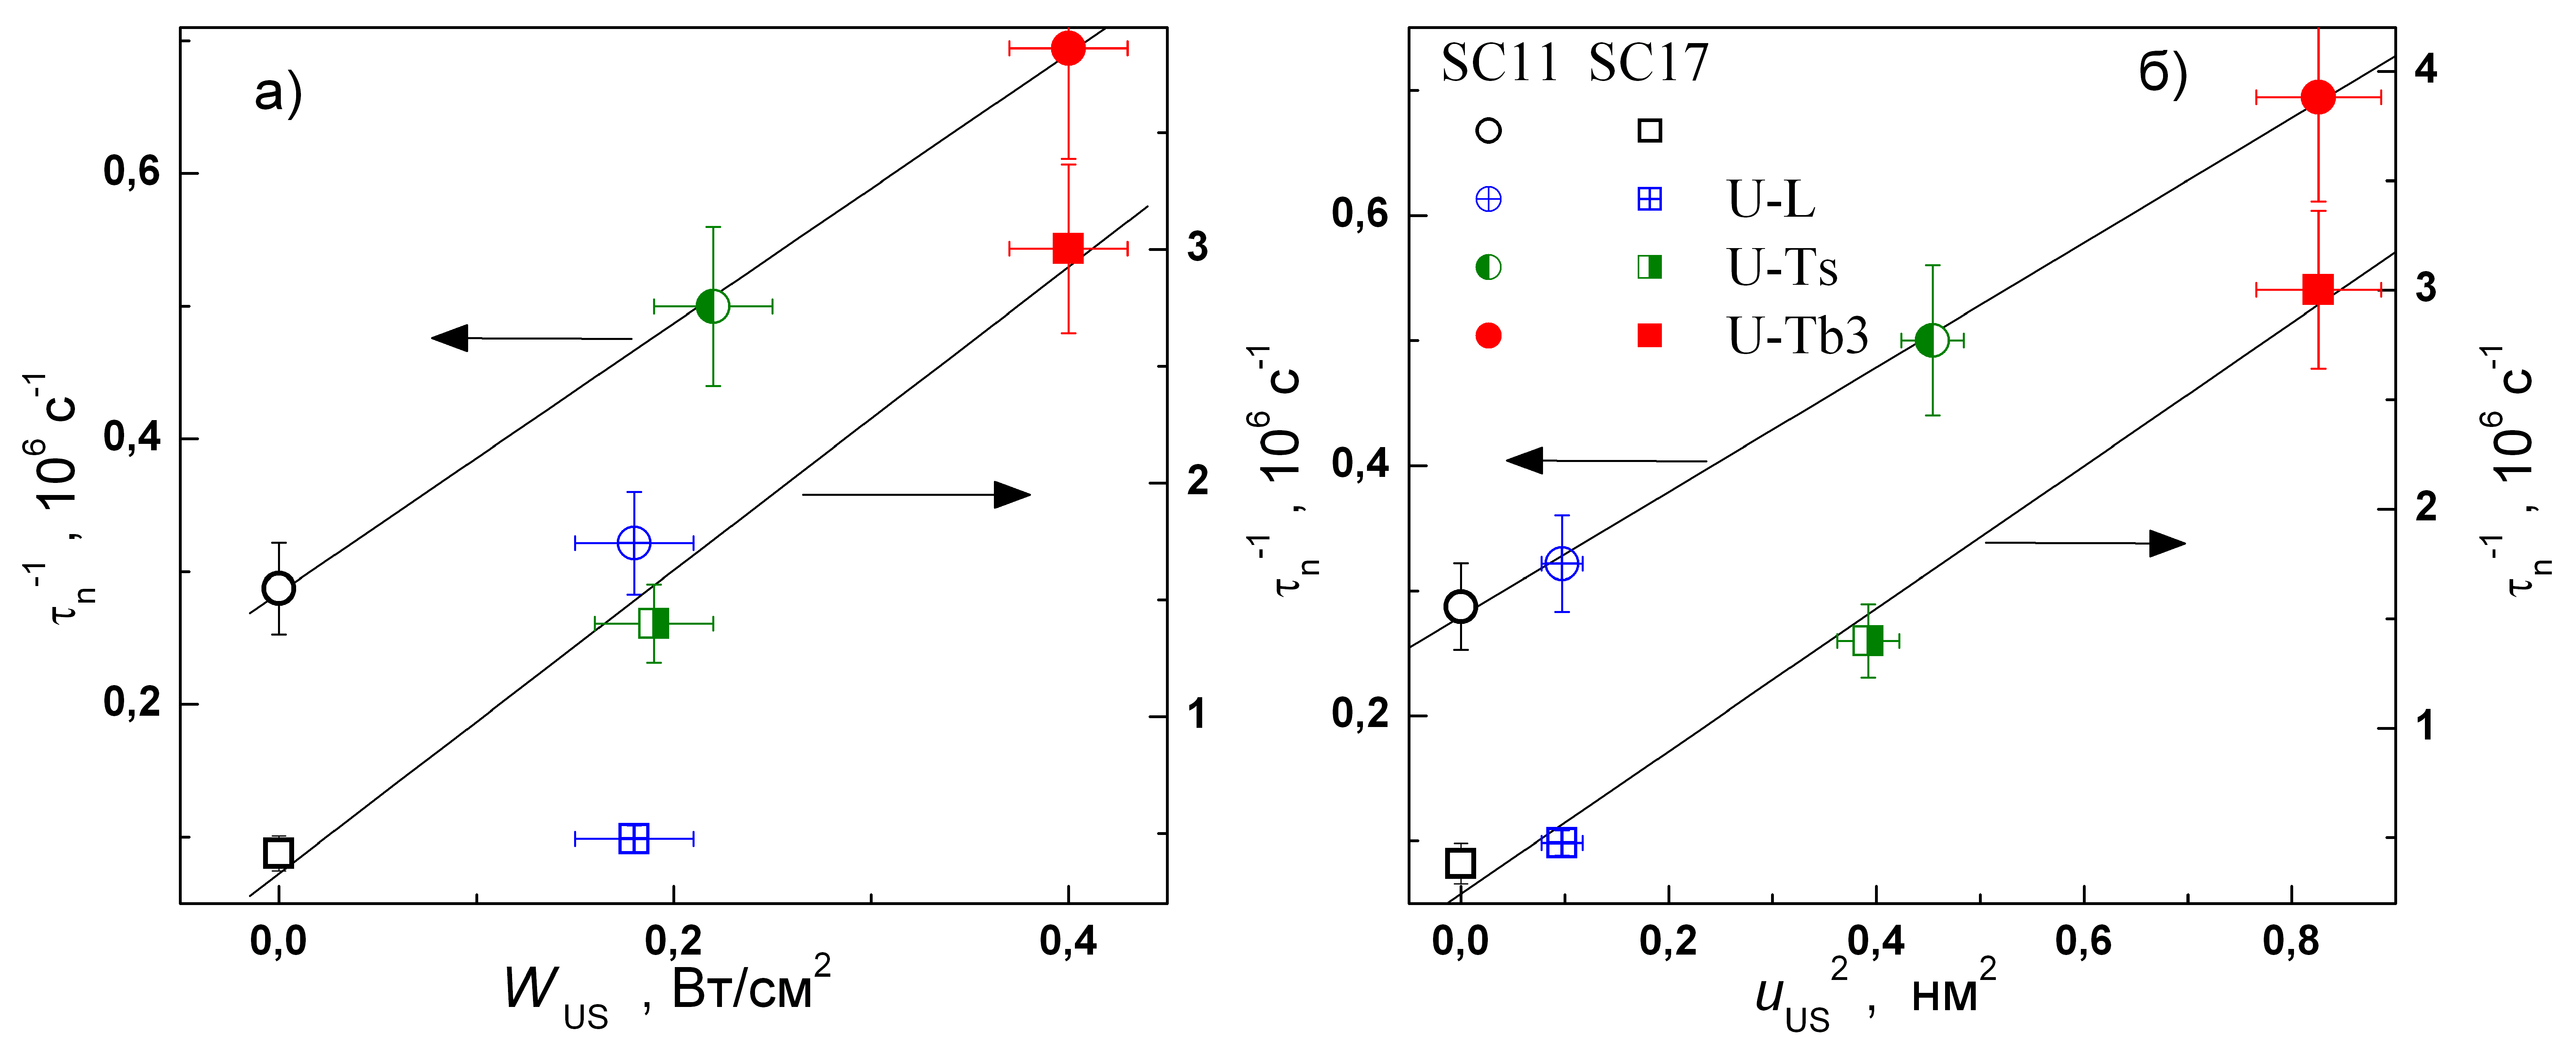
\includegraphics[width=1\textwidth]{figKus}%
%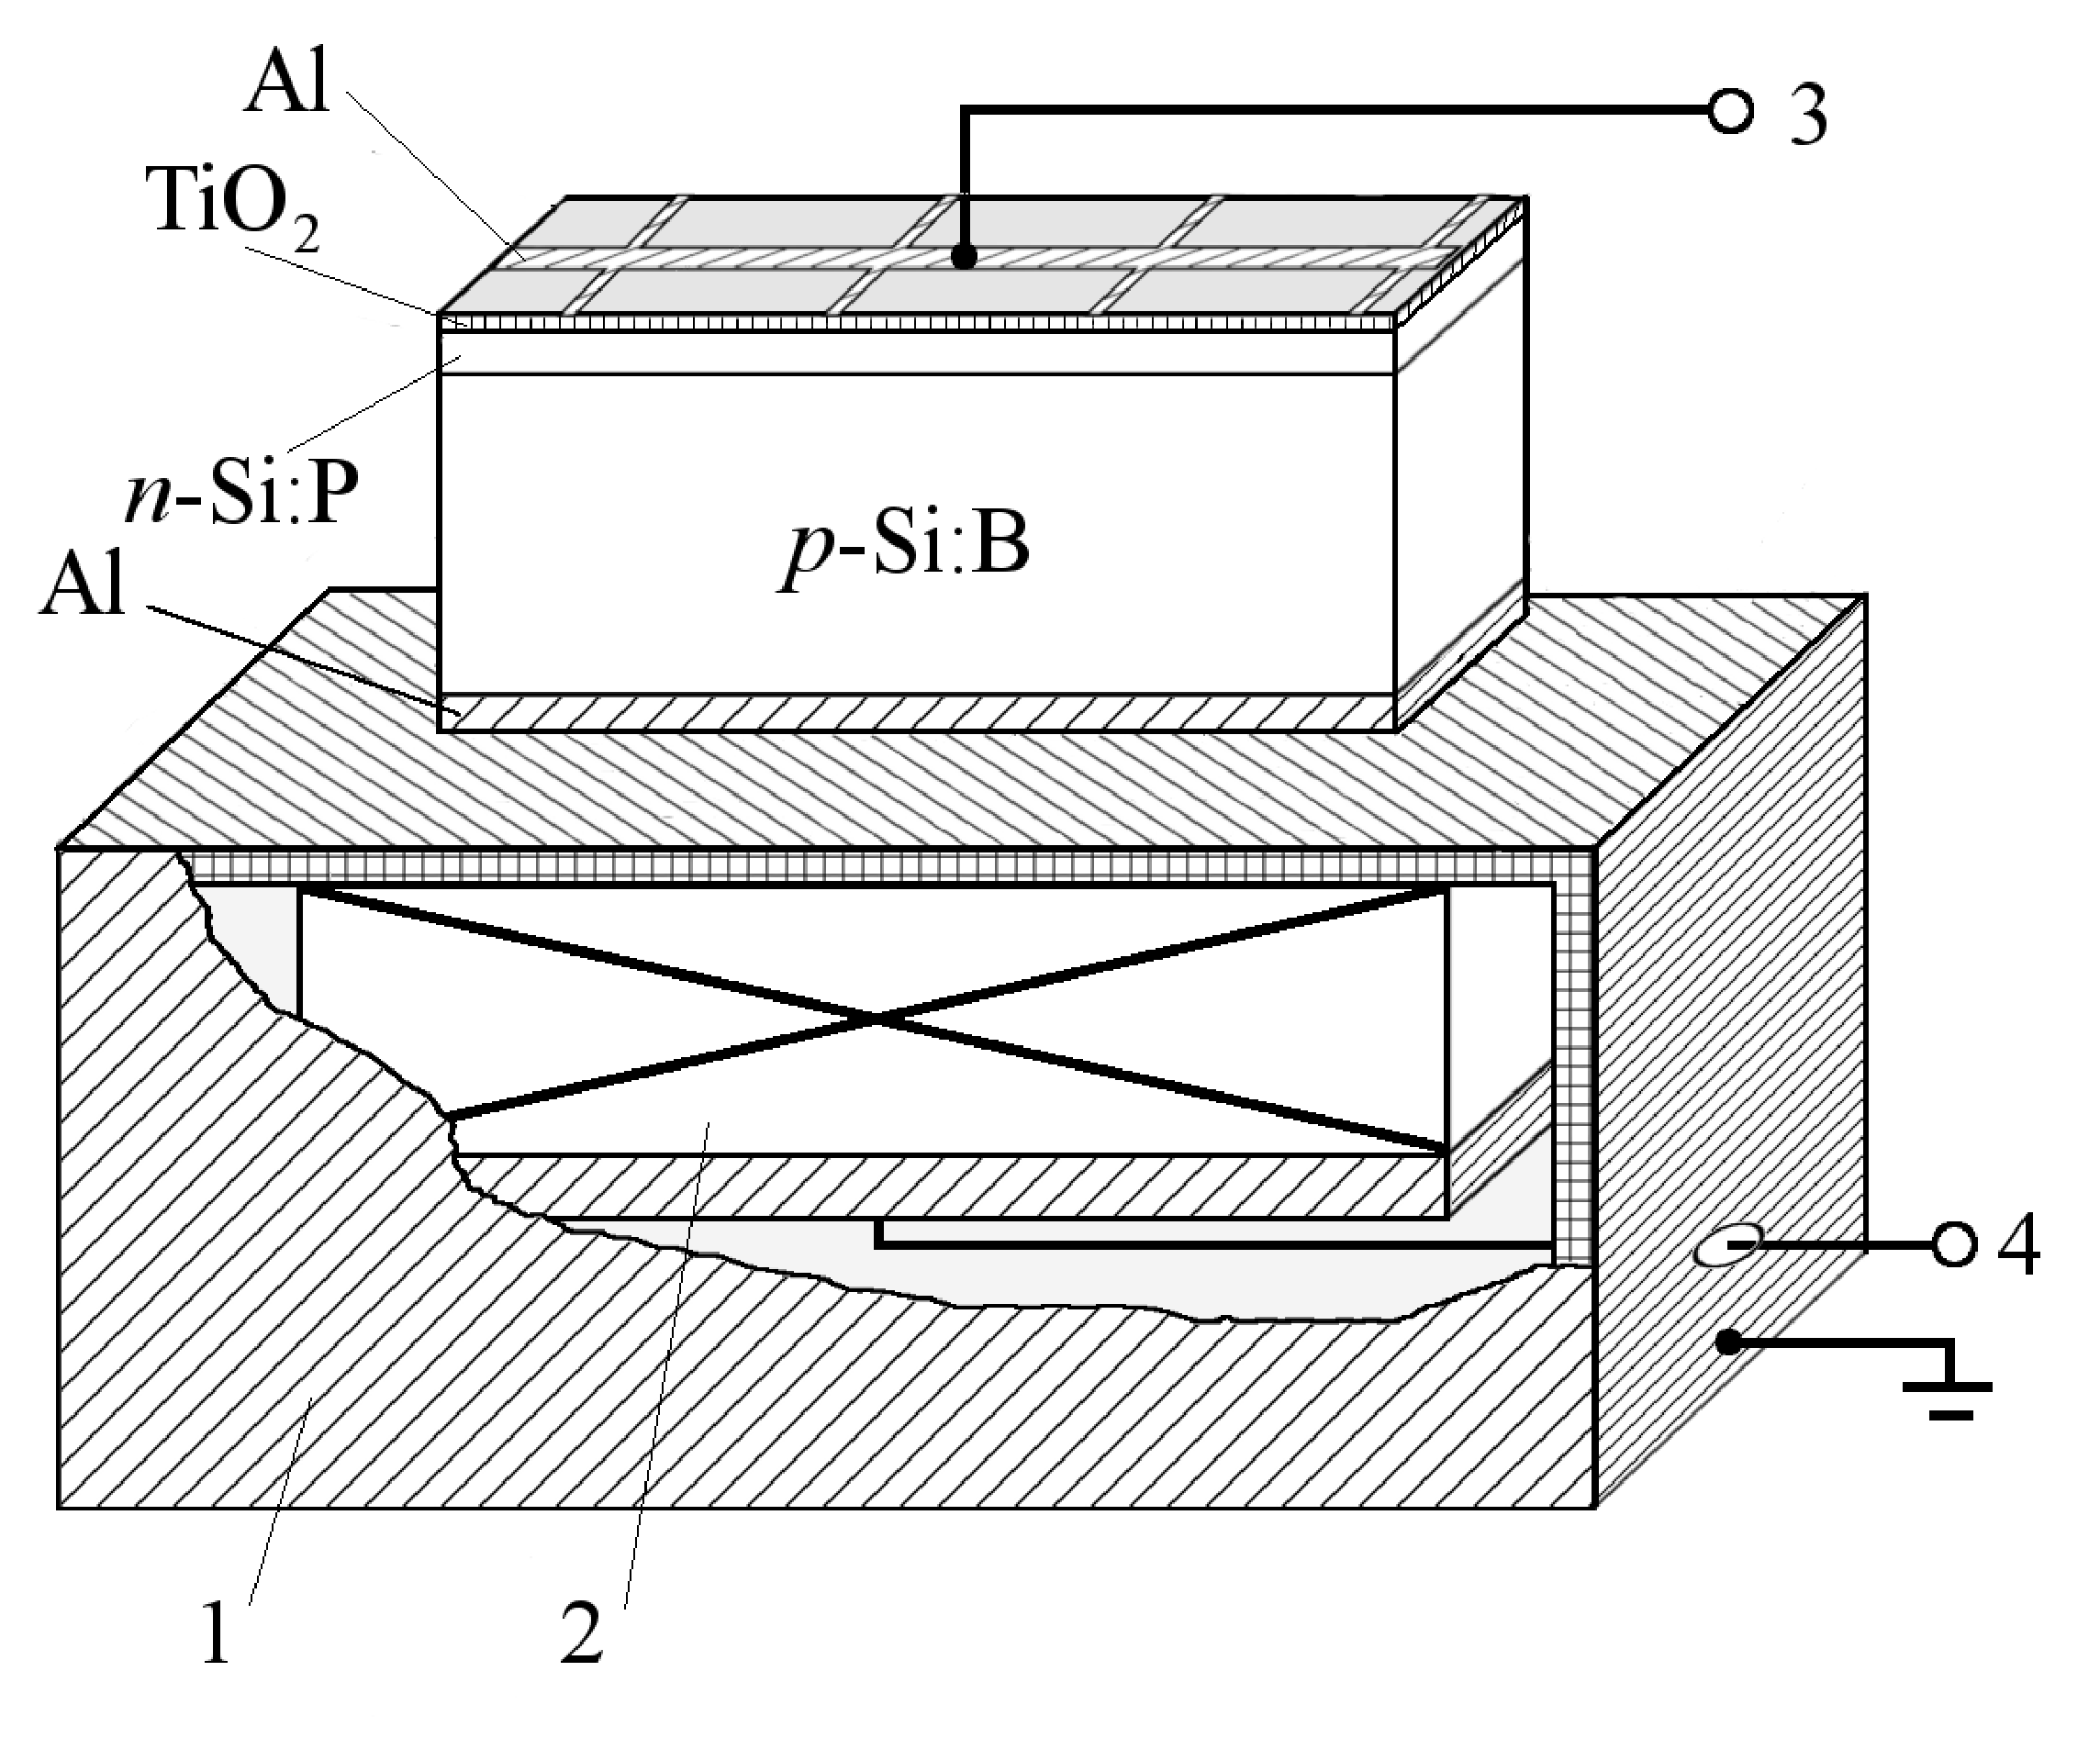
\includegraphics[width=0.4\textwidth]{USL_SC} \hfill
%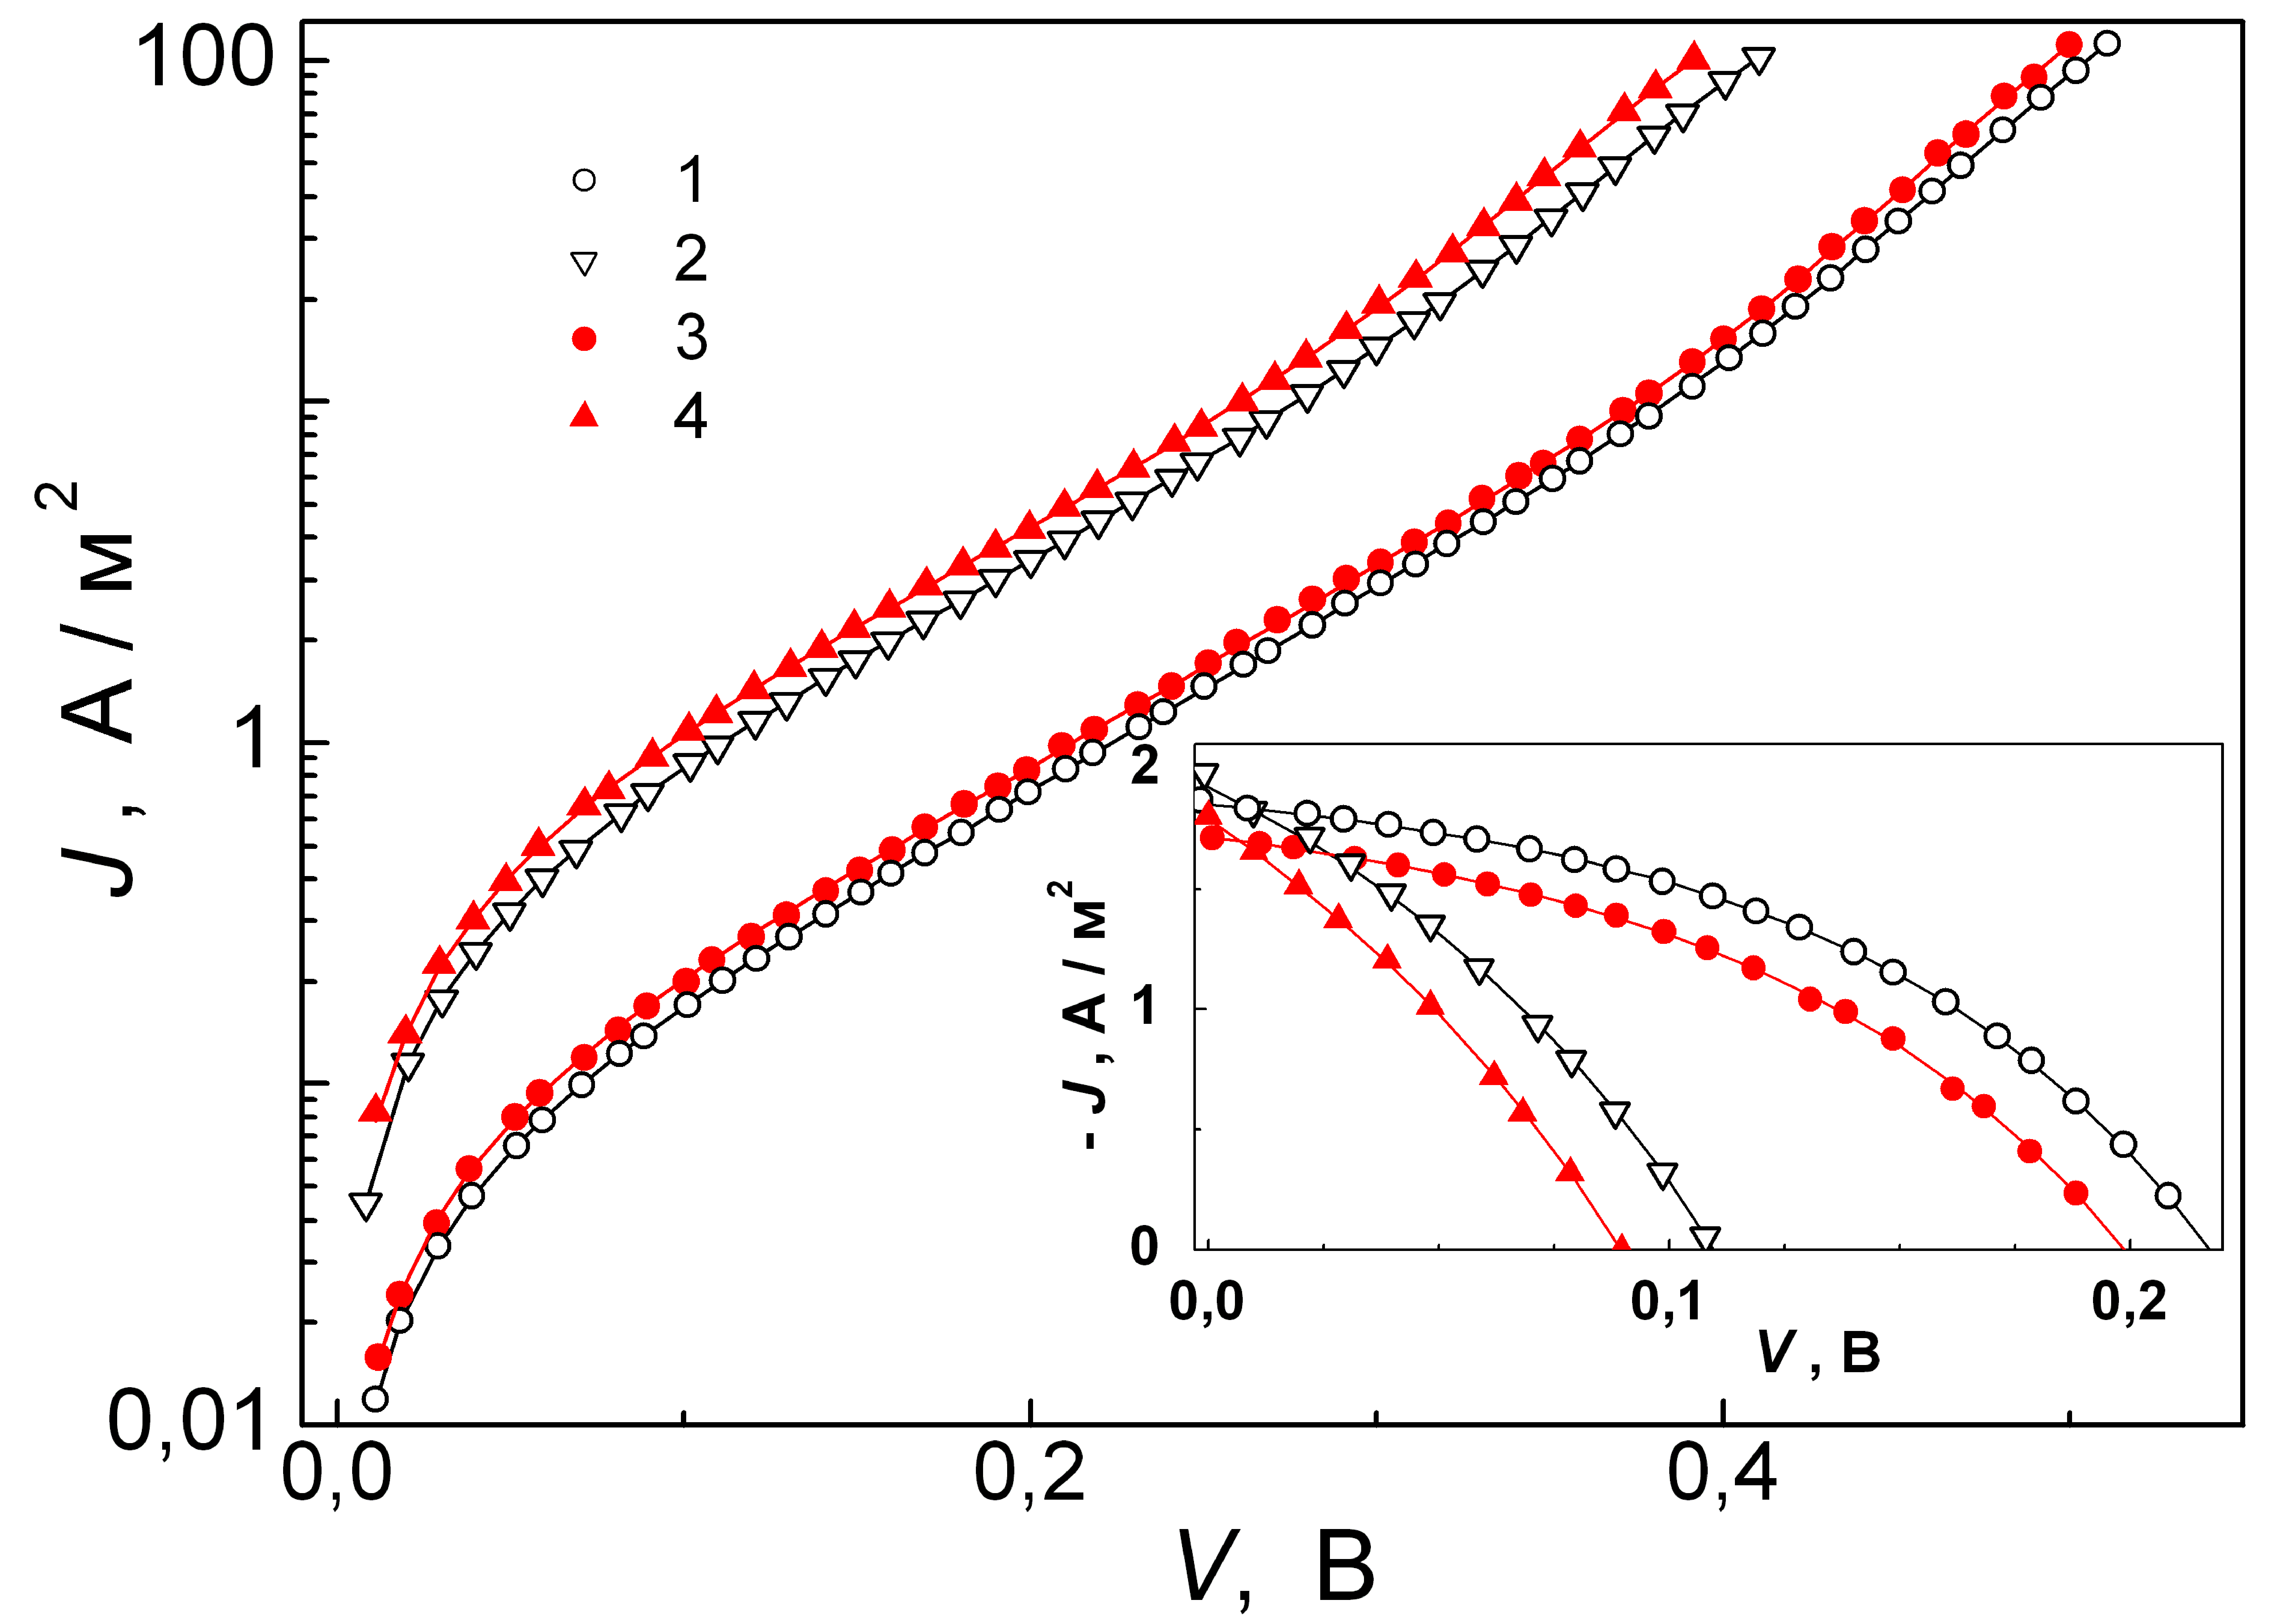
\includegraphics[width=0.55\textwidth]{figSSCIV}
%\caption{\label{USL_SC}
%Зліва --- схема УЗН.
%1 --  екран (алюмінієва фольга, товщина 0,012 мм);
%2 --- п'єзоелектричний перетворювач (LiNbO$_3$);
%3 --- контакти для вимірювання ВАХ;
%4 --- контакти для збудження УЗ.
%Справа --- типові ВАХ, виміряні при температурах 301~K (криві 1 та 2, кола) та 341~K (2 та 4, трикутники)
%за умов УЗН (2, 4, заповнені точки) та для ненавантаженого зразка (1 та 3, порожні точки)
%Точки --- результати вимірів, лінії отримані шляхом апроксимації за формулою (\ref{eqSSCIV}).
%}%
%\end{figure}
%
%
%
%У  \underline{\textbf{третьому розділі}} представлені результати досліджень
%
%
%У  \underline{\textbf{четвертому розділі}} представлені результати досліджень
%
%
%У  \underline{\textbf{п'ятому розділі}} представлені результати досліджень
%
%
%У  \underline{\textbf{шостому розділі}} представлені результати досліджень
%
%
%Во \underline{\textbf{введении}} обосновывается актуальность
%исследований, проводимых в~рамках данной диссертационной работы,
%приводится обзор научной литературы по изучаемой проблеме,
%формулируется цель, ставятся задачи работы, излагается научная новизна
%и практическая значимость представляемой работы. В~последующих главах
%сначала описывается общий принцип, позволяющий ..., а~потом идёт
%апробация на частных примерах: ...  и~... .
%
%
%\underline{\textbf{Первая глава}} посвящена ...
%
% картинку можно добавить так:
%\begin{figure}[ht]
%  \centering
%  \includegraphics [scale=0.27] {latex}
%  \caption{Подпись к картинке.}
%  \label{img:latex}
%\end{figure}
%
%Формулы в строку без номера добавляются так:
%\[
%  \lambda_{T_s} = K_x\frac{d{x}}{d{T_s}}, \qquad
%  \lambda_{q_s} = K_x\frac{d{x}}{d{q_s}},
%\]
%
%\underline{\textbf{Вторая глава}} посвящена исследованию
%
%\underline{\textbf{Третья глава}} посвящена исследованию
%
%Можно сослаться на свои работы в автореферате. Для этого в файле
%\verb!Synopsis/setup.tex! необходимо присвоить положительное значение
%счётчику \verb!\setcounter{usefootcite}{1}!. В таком случае ссылки на
%работы других авторов будут подстрочными.
%\ifnumgreater{\value{usefootcite}}{0}{
%Изложенные в третьей главе результаты опубликованы в~\cite{vakbib1, vakbib2}.
%}{}
%Использование подстрочных ссылок внутри таблиц может вызывать проблемы.
%
%В \underline{\textbf{четвертой главе}} приведено описание
%


%Основні результати представленої роботи полягають у наступному.
%%% Согласно ГОСТ Р 7.0.11-2011:
%% 5.3.3 В заключении диссертации излагают итоги выполненного исследования, рекомендации, перспективы дальнейшей разработки темы.
%% 9.2.3 В заключении автореферата диссертации излагают итоги данного исследования, рекомендации и перспективы дальнейшей разработки темы.
\begin{enumerate}[leftmargin=0cm,itemindent=3em]
  \item Вперше експериментально досліджено вплив ультразвукового навантаження на параметри монокристалічних кремнієвих сонячних елементів у діапазоні температур 290$\div$340~К
  та виявлено оборотну акусто--індуковану деградацію фотоелектричних властивостей, зумовлену зменшенням часу життя носіїв заряду в акустичному полі.
  Виявлено, що в умовах акустичного навантаження збільшується внесок у рекомбінаційні процеси мілкіших рівнів.
  Встановлено, що кисневмісні преципітати ефективно впливають на процеси рекомбінації та беруть участь у акусто--дефектній взаємодії.
  Запропоновано модель акустоактивного комплексного дефекту для пояснення особливостей акусто--індукованих ефектів.
 Виявлено ефект акусто--індукованого зменшення  опору шунтування та запропоновано його пояснення із залученням моделі дислокаційно--індукованого імпедансу.

\item Вперше досліджено вплив ультразвукового навантаження на параметри кремнієвих структур із $p$---$n$--переходом, опромінених реакторними нейтронами та $\gamma$--квантами $^{60}$Co.
      Виявлено, що в опромінених структурах, порівняно з неопроміненими, спостерігається підвищення ефективності акусто--індукованого зменшення  опору шунтування та часу життя неосновних носіїв заряду в базі діода.
      З'ясовано, що акусто--індуковані оборотні зміни фактора неідеальності та часу життя носіїв заряду в області просторового заряду   мають різний знак в опромінених та неопромінених зразках.
      Встановлено, що в нейтронно--опромінених діодах основними акустоактивними центрами є дивакансії,
      а в $\gamma$--опромінених --- комплекс вакансії та міжвузлового кисню
%      виявлені ефекти в нейтронно--опромінених діодах пов'язані зі впливом ультразвуку на стан дивакансій,  тоді як у гамма--опромінених діодах основним акустоактивним центром є комплекс вакансії та міжвузольного кисню.
     Виявлено, що комплекс із міжвузлового вуглецю та міжвузлового кисню не приймає участі в акусто--дефектній взаємодії.

\item  Проведено порівняльний аналіз та тестування 16 основних методів визначення параметрів діодів Шотткі із вольт--амперних характеристик.
         Спираючись на результати тестування методів на експериментальних та синтезованих  ВАХ,
         запропоновано шляхи оптимізації методів Nord, Bohlin та Mikhelashvili з метою збільшення точності розрахунку.
      Запропоновано адаптивну процедуру оптимізації вибору діапазону ВАХ, який використовується для побудови допоміжних функцій при застосуванні аналітичних методів визначення параметрів структур метал---напівпровідник.
       Показано, що така процедура дозволяє суттєво (приблизно на порядок при кімнатних температурах у випадку низького рівня похибок вимірювання) підвищити точність визначення параметрів.

   \item Встановлено, що найефективнішими методами з погляду точності визначення параметрів та швидкості розрахунків є еволюційні алгоритми, метод Gromov із адаптивною процедурою та метод Lee.
    Показано, що використання функції Ламберта при числовому визначенні параметрів діодів Шотткі дозволяє зменшити похибки.
    Розраховані залежності точності визначення послідовного опору, висоти бар'єру Шотткі та фактора неідельності від %величин параметрів та
    рівня випадкових помилок при вимірюванні вольт--амперних характеристик.

   \item
Виявлено, що  перенесення заряду в структурах Al---$n$--$n^+$--Si з бар'єром Шотткі у діапазоні температур 130$\div$330~К при прямому зміщенні відбувається внаслідок термоелектронної емісії через неоднорідний контакт.
%Виконано експериментальне дослідження прямих і зворотних вольт--амперних характеристик структур Al$-n-n^+$--Si---Al з бар'єром Шотткі в діапазоні температур $130\div330$~К.
%Виявлено, що при підвищенні температури спостерігається збільшення висоти бар'єру та зменшення фактора неідеальності та встановлено механізм перенесення заряду із залученням моделі термоелектронної емісії через неоднорідний контакт у всьому діапазоні температур.
%       Показано, що отримані результати можна пояснити у рамках моделі термоелектронної емісії через неоднорідний контакт у всьому діапазоні температур.
        Показано, що при низьких температурах ($T<220$~К) суттєвим стає проходження заряду через області зі зниженим бар'єром і визначено середнє значення висоти бар'єру Шотткі в цих областях.
%          --- $54\pm4$~мВ.
     Виявлено, що при зворотному зміщенні в структурах Al---$n$--$n^+$--Si перенесення заряду відбувається як внаслідок термоелектронної емісії через неоднорідний бар'єр, так і завдяки процесам тунелювання через глибокий центр (міжвузловий атом вуглецю).

\item
%Проведено експериментальне дослідження впливу $\gamma$--ви\-про\-мі\-ню\-ван\-ня $^{60}$Co на електрофізичні параметри структур Al$-n-n^+$--Si---Al.
     Показано, що опромінення $\gamma$-квантами $^{60}$Co структур Al---$n$--$n^+$--Si суттєво підсилює процеси тунелювання носіїв заряду як при прямому зміщенні, так і при зворотному.
     При прямому зміщенні тунельний механізм перенесення заряду стає основним у низькотемпературній області ($T<250$~К),
 при зворотному --- виникає компонента струму, зумовлена багатофононним тунелюванням.
 Виявлено, що висота бар'єру, фактор неідеальності та величина зворотного струму немонотонно змінюються при збільшенні поглинутої дози.
З'ясовано, що при опроміненні з дозою $10^6$~рад зміна
електрофізичних
параметрів відбувається внаслідок накопичення дефектів акцепторного типу на межі метал---напівпровідник та укрупнення патчів, викликаного радіаційно підсиленим дислокаційним ковзанням.
При 
%дозі 
$10^7$~рад
  причинами змін властивостей діодів Шотткі є інтенсифікація процесів тунелювання внаслідок утворення значної кількості радіаційних дефектів та гетерування останніх в областях зі зниженим бар'єром.
Встановлено взаємозв'язок характеру дозової немонотонності зміни висоти бар'єру Шотткі та ступеню неоднорідності контакту.
%Показано, що характер дозової немонотонності зміни висоти бар'єру Шотки різний для   однорідних областей та для всього діоду загалом.


\item
Вперше досліджено динамічний вплив ультразвукового навантаження при кімнатній температурі на параметри кремнієвих діодів Шотткі Al---$n$--$n^+$--Si.
Виявлено
%, що при поширенні акустичних хвиль спостерігаються 
оборотні зменшення висоти бар'єру,
збільшення зворотного струму та струму насичення, тоді як фактор неідеальності практично не змінюється.
З'ясовано, що акустичне навантаження не впливає на процеси прямого та багатофононного тунелювання.
Встановлено, що вплив ультразвука на термоемісійну складову струму структур пояснюється іонізацією дефектів на межі метал---напівпровідник
  внаслідок взаємодії ультразвука з дислокаціями та радіаційними точковими порушеннями періодичності в неопромінених та опромінених структурах, відповідно.

\item
Вперше експериментально досліджено динамічний вплив ультразвукового навантаження в діапазоні частот 8$\div$28~МГц на електричні властивості структур Mo/$n$--$n^{+}$--Si з бар'єром Шотткі за температур 130$\div$330~К.
 Виявлено акусто--індуковані оборотні зміни фактора неідеальності та висоти бар'єру Шотткі, причому зміни немонотонно залежать від температури, а найефективніший вплив ультразвука спостерігається поблизу 200~K.
  Показано, що зі збільшенням частоти ультразвука  спостерігається як загальне підвищення ефективності акустичного впливу на параметри кремнієвих діодів Шотткі,
так і зростання температури максимуму ефективності.
 Використовуючи модель неоднорідного контакту встановлено, що при ультразвуковому навантаженні відбувається збільшення висоти бар'єру як в області розташування патчів, так і за їхніми межами, а також розширюється розподіл параметрів патчів та збільшується їхня ефективна густина.
З'ясовано, що механізм акусто--індукованих змін параметрів структур Mo/$n$--$n^{+}$--Si зумовлений рухом дислокаційних перегинів.
% Показано, що частотні та температурні особливості акустоіндукованих змін параметрів структур Mo/$n$--$n^{+}$--Si можуть бути пояснені в рамках
% моделі поглинання ультразвуку внаслідок руху дислокаційних перегинів.

\item Виявлено ефект оборотного збільшення зворотного струму структур Mo/$n$--$n^{+}$--Si при акустичному навантаженні.
Встановлено, що ефект послаблюється при збільшенні температури та зміщення і посилюється при зростанні частоти ультразвука.
Показано, що основними механізмами зворотного струму є термоелектронна емісія та тунелювання, стимульоване фононами;
в умовах поширення акустичних хвиль відбувається зменшення енергії активації рівнів, що беруть участь у тунелюванні,
густини заповнених інтерфейсних станів та коефіцієнта Пула--Френкеля.

\item Виявлено вплив мікрохвильового опромінення на параметри точкових дефектів у монокристалах $n$--6$H$--SiC, $n$--GaAs та епітаксійних структурах на основі арсеніду ґалію.
Встановлено, що причинами радіаційно--індукованих змін поперечного перерізу захоплення електронів та розташування енергетичних рівнів пасток у забороненій зоні є
збільшення кількості міжвузлових атомів у приповерхневому шарі.
Показано, що радіаційно--індуковані процеси перетворення дефектних комплексів інтенсифікуються за наявності механічних напруг.

\item Вперше експериментально досліджено вплив ультразвукової обробки на параметри структури Au--TiB$_x$--$n$--$n^+$--GaAs з контактом Шотткі
 залежно від частоти та інтенсивності акустичних хвиль.
 Встановлено, що при допороговій (менше 2,5~Вт/см$^2$) інтенсивності ультразвука відбувається збільшення однорідності параметрів арсенід--ґалієвих діодів Шотткі, створених в єдиному технологічному процесі, зумовлене
 акусто--стимульованою дифузією  дефектів.



\item Виявлено, що  ультразвукова обробка викликає зменшення концентрації та звуження енергетичного спектра радіаційних дефектів у системи   Si--SiO$_2$.
    Показано, що причиною ефекту є акусто--індукована дифузія атомів водню та кисню.

%  На основе анализа \ldots
%  \item Численные исследования показали, что \ldots
%  \item Математическое моделирование показало \ldots
%  \item Для выполнения поставленных задач был создан \ldots
\end{enumerate}





%\begin{center}%
{\textbf{\MakeUppercase{\authorbibtitle}} }
\end{center}%

\begin{center}%
\emph{Наукові праці, в яких опубліковано основні наукові результати дисертації}
\end{center}%
\begin{enumerate}[label=\arabic*.,leftmargin=1cm,itemindent=0cm]
%\setcounter{enumi}{25}
\item
Acousto--defect interaction in irradiated and non--irradiated silicon
  $n^+$--$p$ structure~/ O.~Ya.~Olikh, A.~M.~Gorb, R.~G.~Chupryna,
  O.~V.~Pristay-Fenenkov~// \emph{J. Appl. Phys.} --- 2018. --- 
 Vol. 123, no.~16. --- P.~161573--1--161573--12.

\item
\emph{Olikh,~O.Ya.} Acoustically driven degradation in single crystalline
  silicon solar cell~/ O.Ya.~Olikh~// \emph{Superlattices Microstruct.} ---
  2018. --- 
  Vol. 117. ---
  P.~173--188.

\item
\emph{Olikh,~O.} On the mechanism of ultrasonic loading effect in
  silicon--based {S}chottky diodes~/ O.~Olikh, K.~Voytenko~//
  \emph{Ultrasonics}. ---
  2016. ---  Vol.~66, no.~1. ---
  P.~1--3.

\item
Effect of ultrasound on reverse leakage current of silicon {S}chottky barrier
  structure~/ O.~Ya.~Olikh, K.~V.~Voytenko, R.~M.~Burbelo, Ja.~M.~Olikh~//
  \emph{Journal of Semiconductors}. ---
  2016. --- 
  Vol.~37, no.~12. ---
  P.~122002--1--122002--7.

\item
\emph{Olikh,~O.~Ya.} Review and test of methods for determination of the
  {S}chottky diode parameters~/ O.~Ya.~Olikh~// \emph{J. Appl. Phys.} ---
  2015. --- 
  Vol. 118, no.~2. ---
  P.~024502--1--024502--14.

\item
\emph{Olikh,~O.~Ya.} Ultrasound influence on {I}--{V}--{T} characteristics
  of silicon {S}chottky barrier structure~/ O.~Ya.~Olikh, K.~V.~Voytenko,
  R.~M.~Burbelo~// \emph{J. Appl. Phys.} ---
  2015. --- 
  Vol. 117, no.~4. ---
  P.~044505--1--044505--7.

\item
\emph{Olikh,~O.}. Reversible influence of ultrasound on
  $\gamma-$irradiated {M}o/n-{S}i {S}chottky barrier structure~/ O.~Olikh~//
  \emph{Ultrasonics}. ---
  2015. --- 
  Vol.~56. ---
  P.~545--550.

\item
Особливості дислокаційного поглинання
  ультразвуку в безсубблочних кристалах
  {C}d$_{0,2}${H}g$_{0,8}${T}e~/ І.~О.~Лисюк, Я.~М.~Оліх,
  О.~Я.~Оліх, Г.~В.~Бекетов~// \emph{УФЖ}. ---
  2014. ---
  Т.~59, {№}~1. ---
  {С.}~50--57.

\item
\emph{Olikh,~O.~Ya.} Non-Monotonic $\gamma-$Ray Influence on {M}o/n-{S}i
  {S}chottky Barrier Structure Properties~/ O.~Ya.~Olikh~// \emph{IEEE
  Trans. Nucl. Sci.} ---
  2013. --- 
  Vol.~60, no.~1. ---
  P.~394--401.

\item
\emph{Оліх,~О.~Я.} Особливості впливу
  ультразвуку на перенесення заряду в
  кремнієвих структурах з бар’єром {Ш}отки
  залежно від дози $\gamma$--опромінення~/
  О.~Я.~Оліх~// \emph{Сенсорна електроніка і
  мікросистемні технології}. ---
  2013. ---
  Т.~10, {№}~1. ---
  {С.}~47--55.

\item
\emph{Олих,~О.~Я.} Влияние ультразвукового
  нагружения на протекание тока в
  структурах {M}o/n--n$^+$--{S}i c барьером {Ш}оттки~/
  О.~Я.~Олих~// \emph{Физика и техника
  полупроводников}. ---
  2013. ---
  Т.~47, {№}~7. ---
  {С.}~979--984.

\item
\emph{Оліх,~О.~Я.} Особливості перенесення
  заряду в структурах {M}o/n--{S}i з бар’єром
  {Ш}отки~/ О.~Я.~Оліх~// \emph{УФЖ}. ---
  2013. ---
  Т.~58, {№}~2. ---
  {С.}~126--134.

\item
\emph{Олих,~О.~Я.} Особенности динамических
  акустоиндуцированных изменений
  фотоэлектрических параметров кремниевых
  солнечных элементов~/ О.~Я.~Олих~//
  \emph{Физика и техника полупроводников}. ---
  2011. ---
  Т.~45, {№}~6. ---
  {С.}~816--822.

\item
\emph{Оліх,~Я.~М.} Інформаційний чинник
  акустичної дії на структуру дефектних
  комплексів у напівпровідниках~/ Я.~М.~Оліх,
  О.~Я.~Оліх~// \emph{Сенсорна електроніка і
  мікросистемні технології}. ---
  2011. ---
  Т. 2(8), {№}~2. ---
  {С.}~5--12.

\item
\emph{Оліх,~О.~Я.} Особливості впливу
  нейтронного опромінення на динамічну
  акустодефектну взаємодію у кремнієвих
  сонячних елементах~/ О.~Я.~Оліх~// \emph{УФЖ}.
  ---
  2010. ---
  Т.~55, {№}~7. ---
  {С.}~770--776.


\item
Ultrasonically Recovered Performance of $\gamma-$Irradiated Metal-Silicon
  Structures~/ A.M.~Gorb, O.A.~Korotchenkov, O.Ya~Olikh, A.O.~Podolian~//
  \emph{IEEE Trans. Nucl. Sci.} ---
  2010. --- 
  Vol.~57, no.~3. ---
  P.~1632--1639.

\item
\emph{Олих,~О.~Я.} Изменение активности
  рекомбинационных центров в кремниевых
  p--n--структурах в условиях акустического
  нагружения~/ О.~Я.~Олих~// \emph{Физика и
  техника полупроводников}. ---
  2009. ---
  Т.~43, {№}~6. ---
  {С.}~774--779.

\item
\emph{Оліх,~О.~Я.} Робота кремнієвих сонячних
  елементів в умовах акустичного
  навантаження мегагерцового діапазону~/
  О.~Я.~Оліх, Р.~М.~Бурбело, М.~К.~Хіндерс~//
  \emph{Сенсорна електроніка і
  мікросистемні технології}. ---
  2007. ---
  Т.~4, {№}~3. ---
  {С.}~40--45.

\item
%\emph{Olikh,~O.Ya.} The Dynamic Ultrasound Influence on Diffusion and Drift
%  of the Charge Carriers in Silicon p--n Structures~/ O.Ya.~Olikh, R.~Burbelo,
%  M.~Hinders~// Semiconductor Defect Engineering --- Materials, Synthetic,
%  Structures and Devices II~/ Ed. by S.~Ashok, P.~Kiesel, J.~Chevallier,
%  T.~Ogino. ---
%  Vol.~994 of \emph{Materials Research Society Symposium
%  Proceedings}. ---
%  Warrendale, PA: 2007. ---
%  P.~269--274.
\emph{Burbelo,~R.~M.} The Dynamic Ultrasound Influence on the Diffusion
  and Drift of the Charge Carriers in Silicon p-n Structures~/
  R.~M.~Burbelo, O.~Y.~Olikh, M.~K.~Hinders~// \emph{MRS
  Proceedings}. ---
 2007. ---
Vol. 994. ---
P.~0994–F03--11.

\item
\emph{Олих,~О.~Я.} Акустостимулированные
  коррекции вольт--амперных характеристик
  арсенид--галлиевых структур с контактом
  {Ш}оттки~/ О.~Я.~Олих, Т.~Н.~Пинчук~//
  \emph{Письма в Журнал Технической Физики}.
  ---
  2006. ---
  Т.~32, {№}~12. ---
  {С.}~22--27.

\item
\emph{Конакова,~Р.В.} Влияние микроволновой
  обработки на уровень остаточной
  деформации и параметры глубоких уровней
  монокристаллах карбида кремния~/
  Р.В.~Конакова, П.М.~Литвин, О.Я.~Олих~//
  \emph{Физика и химия обработки материалов}.
  ---
  2005. ---
  {№}~2. ---
  {С.}~19--22.


\item
\emph{Конакова,~Р.В.} Влияние микроволновой
  обработки на глубокие уровни
  монокристаллов {G}a{A}s и {S}i{C}~/ Р.В.~Конакова,
  П.М.~Литвин, О.Я.~Олих~// \emph{Петербургский
  журнал электроники}. ---
  2004. ---
  {№}~1. ---
  {С.}~20--24.

\item
\emph{Olikh,~Ja.~М.} Active ultrasound effects in the future usage in
  sensor electronics~/ Ja.~М.~Olikh, O.Ya.~Olikh~// \emph{Сенсорна
  електроніка і мікросистемні технології}.
  ---
  2004. ---
  Т.~1, {№}~1. ---
  {С.}~19--29.

\item
\emph{Olikh,~O.Ya.} Acoustoelectric transient spectroscopy of microwave
  treated {G}a{A}s--based structures~/ O.Ya.~Olikh~// \emph{Semiconductor
  Physics, Quantum Electronics \& Optoelectronics}. ---
  2003. ---
  Vol.~6, no.~4. ---
  P.~450--453.

\item
\emph{Оліх,~О.Я.} Акустостимульовані
  динамічні ефекти в сонячних елементах на
  основі кремнію~/ О.Я.~Оліх~// \emph{Вісник
  Київського ун-ту, Сер.: Фізико-математичні
  науки}. ---
  2003. ---
  {№}~4. ---
  {С.}~408--414.
\end{enumerate}

\begin{center}%
\emph{Наукові праці, які засвідчують апробацію матеріалів дисертації}
\end{center}%
\begin{enumerate}[label=\arabic*.,leftmargin=2em,itemindent=0cm]
\setcounter{enumi}{25}
\item
\emph{Оліх,~О.~Я.} Ефекти активного
  ультразвуку в напівпровідникових
  кристалах~/ О.~Я.~Оліх~// 1--а {У}країнська
  наукова конференція з фізики
  напівпровідників, {О}деса, {У}країна. ---
  Т.~1. ---
  Одеса: 2002. ---
  {С.}~80.

\item
Влияние {СВЧ} облучения на остаточный
  уровень внутренних механических
  напряжений и параметры глубоких уровней в
  эпитак-сиальных структурах {G}a{A}s~/
  Р.~В.~Конакова, А.~Б.~Камалов, О.~Я.~Олих
  {и~др.}~// Труды {III} международной
  конференции <<{Р}адиационно--термические
  эффекты и процессы в неорганических
  материалах>>, {Т}омск, {Р}оссия. ---
  Томск: 2002. ---
  {С.}~338--339.

\item
\emph{Оліх,~О.~Я.} Про роль теплових і
  деформаційних механізмів дії ультразвуку
  на роботу кремнієвих сонячних елементів~/
  О.~Я.~Оліх~// Міжнародна науково--технічна
  конференція <<{С}енсорна електроніка і
  мікросистемні технології {СЕМСТ}--1>>,
  {О}деса, {У}країна. Тези доповідей. ---
  Одеса: 2004. ---
  {С.}~163.

\item
\emph{Olikh,~O.} Investigation of microwave treated epitaxial {G}a{A}s
  structures by acoustoelectric method~/ O.~Olikh~// 2004 {IEEE}
  {I}nternational {U}ltrasonics, {F}erroelectrics and {F}requency {C}ontrol
  {J}oint 50$^{th}$ {A}nniversary {C}onference. Montreal, {C}anada. Abstracts.
  ---
  Montreal: 2004. ---
  P.~230--231.

\item
\emph{Олих,~О.~Я.} Влияние {СВЧ} облучения на
  остаточный уровень внутренних
  механических напряжений и параметры
  глубоких уровней в эпитак-сиальных
  структурах {G}a{A}s~/ О.~Я.~Олих~// Труды девятой
  международной научно--технической
  конференции <<{А}ктуальные проблемы
  твердотельной электроники и
  микроэлектроники>>, {Д}ивноморское,
  {Р}оссия. ---
  Дивноморское: 2004. ---
  {С.}~278--279.

\item
Influence of acoustic wave on forming and characteristics of silicon p--n
  junction~/ J.~Olikh, A.~Evtukh, B.~Romanyuk, O.~Olikh~// 2005 {IEEE}
  {I}nternational {U}ltrasonics {S}ymposium and {S}hort {C}ourses. Rotterdam,
  {N}etherlands. Abstracts. ---
  Rotterdam: 2005. ---
  P.~542.

\item
\emph{Olikh,~O.} Dynamic ultrasound effects in silicon solar sell~/
  O.~Olikh, R.~Burbelo, Hinders~M.~// 2007 {I}nternational {C}ongress on
  {U}ltrasonics. {P}rogram and {B}ook of {A}bstracts. {V}ienna, {A}ustria. ---
  Vienna: 2007. ---
  P.~94.

\item
\emph{Olikh,~O.} Influence of the ultrasound treatment on
  {A}u-{T}i{B}--n--n$^+$--{G}a{A}s structure electrical properties~/
  O.~Olikh~// 2007 {I}nternational {C}ongress on {U}ltrasonics. {P}rogram and
  {B}ook of {A}bstracts. {V}ienna, {A}ustria. ---
  Vienna: 2007. ---
  P.~94.

\item
\emph{Olikh,~O.} The Dynamic Ultrasound In-fluence on Diffusion and Drift of
  the Charge Carriers in Silicon p--n Structures~/ O.~Olikh, R.~Burbelo,
  M.~Hinders~// {MRS} 2007 {S}pring {M}eeting, {S}ymposium {F}: {S}emiconductor
  {D}efect {E}ngineering --- {M}aterials, {S}ynthetic {S}tructures, and
  {D}evices {II}. San {F}rancisco, {USA}. ---
  San {F}rancisco: 2007. ---
  P.~3.11.

\item
\emph{Оліх,~О.~Я.} Робота кремнієвих сонячних
  елементів в умовах акустичного
  навантаження мегагерцового діапазону~/
  О.~Я.~Оліх~// {ІІІ} {У}країнська наукова
  конференція з фізики напівпровідників
  {УНКФН}--3, {О}деса, {У}країна. Тези доповідей.
  ---
  Одеса: 2007. ---
  {С.}~322.

\item
\emph{Оліх,~О.~Я.} Вплив ультразвукової
  обробки на вольт--амперні характеристики
  опромінених кремнієвих структур~/
  О.~Я.~Оліх, А.~М.~Горб~// {VІ} {М}іжнародна
  школа--конференція <<Актуальні проблеми
  фізики напівпровідників>>, {Д}рогобич,
  {У}країна. Тези доповідей. ---
  Дрогобич: 2008. ---
  {С.}~114.

\item
\emph{Оліх,~О.~Я.} Акустичні збурення
  дефектної підсистеми кремнієвих
  p--n--структур~/ О.~Я.~Оліх~// {VІ} {М}іжнародна
  школа--конференція <<Актуальні проблеми
  фізики напівпровідників>>, {Д}рогобич,
  {У}країна. Тези доповідей. ---
  Дрогобич: 2008. ---
  {С.}~174.


\item
\emph{Оліх,~О.~Я.} Особливості механізму
  ультразвукового впливу на
  фото--електричний струм у
  нейтронно--опромінених {S}i--p--n--структурах~/
  О.~Я.~Оліх~// {IV} {У}країнська наукова
  конференція з фізики напівпровідників,
  {З}апоріжжя, {У}країна. Тези доповідей. ---
  Т.~2. ---
  {З}апоріжжя: 2009. ---
  {С.}~59.

  \item
\emph{Olikh,~O.} Ultrasound influence on the recombination centers in
  silicon p-n--structures~/ O.~Olikh~// 13th International Conference on
  Defects --- Recognition, Imaging and Physics in Semiconductors. Wheeling,
  {USA}. Final program. ---
Wheeling: 2009. ---
P.~9--10.


\item
\emph{Оліх,~Я.~М.} Про можливості практичного
  застосування ультразвуку для керування
  характеристиками перетворювачів
  сонячної енергії~/ Я.~М.~Оліх, О.~Я.~Оліх~//
  Четверта міжнародна науково--практична
  конференція <<Матеріали електронної
  техніки та сучасні інформаційні
  технології>>, {К}ременчук, {У}країна. Тези
  доповідей. ---
  {К}ременчук: 2010. ---
  {С.}~147--148.

\item
\emph{Оліх,~О.~Я.} Немонотонний вплив
  $\gamma$--опромінення на електричні
  властивості кремнієвих структур з
  бар’єром {Ш}отки~/ О.~Я.~Оліх, С.~В.~Онисюк~//
  {VІI} {М}іжнародна школа--конференція
  <<Актуальні проблеми фізики
  напівпровідників>>, {Д}рогобич, {У}країна.
  Тези доповідей. ---
  Дрогобич: 2010. ---
  {С.}~171--172.

\item
\emph{Оліх,~О.~Я.} Особливості динамічного
  ультразвукового впливу на
  $\gamma$--опромінені кремнієві $m-s-$структури~/
  О.~Я.~Оліх, С.~В.~Онисюк~// Збірник тез {V}
  {У}країнської наукової конференції з
  фізики напівпровідників {УНКФН}--5,
  Ужгород, {У}країна. ---
  Ужгород: 2011. ---
  {С.}~339--340.

\item
\emph{Оліх,~О.~Я.} Вплив ультразвуку на
  термоемісійні процеси в Mo/n--n$^+$--Si
  структурах~/ О.~Я.~Оліх~// Матеріали
  {В}сеукраїнської наукової конференції
  <<Актуальні проблеми теоретичної,
  експериментальної та прикладної фізики>>,
  {Т}ернопіль, {У}країна. ---
  Тернопіль: 2012. ---
  {С.}~101--103.

\item
\emph{Olikh,~O.~Ya.} Reversible Alteration of Reverse Current in Mo/n--Si
  Structures Under Ultrasound Loading~/ O.~Ya.~Olikh, Ya.~M.~Olikh~//
  Фізика і технологія тонких плівок та
  наносистем. {М}атеріали {ХІV} Міжнародної
  конференції~/ {Під ред. }Д.М.~Фреїкa. ---
  Івано--Франківськ: Видавництво
  {П}рикарпатського національного
  університету імені {В}асиля {С}тефаника,
  2013. ---
  {С.}~322.

\item
\emph{Olikh,~O.~Ya.} Modification of reverse current in the Mo/n--Si
  structures under conditions of ultrasonic loading~/ O.~Ya.~Olikh,
  K.~V.~Voytenko~// {VІІI} {I}nternational school--conference <<Actual
  problems of semiconductor physics>>, {D}rohobych, {U}kraine. Abstract book.
  ---
  Drohobych: 2013. ---
  P.~101--102.

\item
\emph{Olikh,~Ya.~M.} About acoustical--stimulated a self--organization
  defect structures in semiconductor during ion implantation~/ Ya.~M.~Olikh,
  O.~Ya.~Olikh~// International research and practice conference
  <<Nanotechnology and nanomaterials>>, {B}ukovel, {U}kraine. Abstract book.
  ---
  Bukovel: 2013. ---
  P.~240.

\item
\emph{Оліх,~О.~Я.} Вплив $\gamma$--опромінення на
  механізм перенесення заряду в структурах
  Mo/n--Si~/ О.~Я.~Оліх~// {VІ} {У}країнська наукова
  конференція з фізики напівпровідників
  {УНКФН}--6. Чернівці, {У}країна. Тези
  доповідей. ---
  Чернівці: 2013. ---
  {С.}~121--122.

\item
\emph{Olikh,~Ya.} New approach to ultrasonic absorption in subgrain--free
  {C}d$_{0,2}${H}g$_{0,8}${T}e crystals~/ Ya.~Olikh, I.~Lysyuk, O.~Olikh~//
  2014 {IEEE} {I}nternational {U}ltrasonics {S}ymposium. Chicago, {I}llinois,
  {USA}. Abstract book. ---
  Chicago: 2014. ---
  P.~439--440.

\item
\emph{Olikh,~O.} Ultrasonically induced effects in {S}chottky barrier
  structure depending on a $\gamma$--irradiation~/ O.~Olikh~// 2014 {IEEE}
  {I}nternational {U}ltrasonics {S}ymposium. Chicago, {I}llinois, {USA}.
  Abstract book. ---
  Chicago: 2014. ---
  P.~645--646.

\item
\emph{Оліх,~О.~Я.} Характеризація
  $\gamma$--опромінених кремнієвих p--n--структур
  методом диференційних коефіцієнтів~/
  О.~Я.~Оліх, О.~В.~Пристай~// 6--та Міжнародна
  науково--технічна конференція <<{С}енсорна
  електроніка і мікросистемні технології>>,
  {О}деса, {У}країна. Тези доповідей. ---
  Одеса: 2014. ---
  {С.}~193.

\item
\emph{Olikh,~O.Ya.}. Ultrasonic Loading Effects on Silicon--based Schottky
  Diodes~/ O.Ya.~Olikh, K.~V.~Voytenko~// 2015 {I}nternational {C}ongress on
  {U}ltrasonics. Metz, {F}rance. Abstract book. ---
  Metz: 2015. ---
  P.~225.

\item
\emph{Оліх,~О.~Я.} Порівняння ефективності
  методів визначення параметрів діодів
  {Ш}отки~/ О.~Я.~Оліх~// Сучасні проблеми
  фізики конденсованого стану: {П}раці {IV}--ї
  міжнародної конференції. {К}иїв, {У}країна.
  ---
  Київ: 2015. ---
  {С.}~32--34.

\item
Ультразвукова модифікація стимульованого
  фононами тунелювання у кремнієвих діодах
  Шотки~/ О.~Я.~Оліх, К.~В.~Войтенко,
  Р.~М.~Бурбело, Я.~М.~Оліх~// {VІI} {У}країнська
  наукова конференція з фізики
  напівпровідників {УНКФН}--7. Дніпро,
  {У}країна. Тези доповідей. ---
  Дніпро: 2016. ---
  {С.}~190--191.

\item
\emph{Оліх,~О.~Я.} Акусто--керована
  модифікація властивостей кремнієвих
  фотоелектроперетворювачів~/ О.~Я.~Оліх~//
  Перспективні напрямки сучасної
  електроніки, інформаційних і
  комп’ютерних систем. Тези доповідей на
  {ІІ} Всеукраїнській науково--практичній
  конференції {МЕІСS}--2017. Дніпро, {У}країна. ---
  Дніпро: 2017. ---
  {С.}~302--303.

\end{enumerate}


%
%\begin{center}
%\section*{\MakeUppercase{анотація}}
%\end{center}
%
%\textbf{\thesisAuthorFIO~\thesisTitle.} --- Рукопис.
%
%\abstractBegin
%
%\keywords
%
%
%\begin{center}
%{\section*{\MakeUppercase{АННОТАЦИЯ}}}
%\end{center}
%
%\textbf{\thesisAuthorFIOru~\thesisTitleRu.} --- Рукопись.
%
%\abstractBeginRu
%
%\keywordsRu
%
%
%\begin{center}
%{\section*{\MakeUppercase{ABSTRACT}}}
%\end{center}
%
%\textbf{\thesisAuthorFIOen~\thesisTitleEn.} ---  Manuscript.
%
%\abstractBeginEn
%
%\keywordsEn


%
%\begin{center}
%\section*{\MakeUppercase{АННОТАЦИЯ}}
%\end{center}
%ооо
%
%\begin{center}
%\section*{\MakeUppercase{ABSTRACT}}
%\end{center}
%

%\newpage
%При использовании пакета \verb!biblatex! список публикаций автора по теме
%диссертации формируется в разделе <<\publications>>\ файла
%\verb!../common/characteristic.tex!  при помощи команды \verb!\nocite!
%
%\ifdefmacro{\microtypesetup}{\microtypesetup{protrusion=false}}{} % не рекомендуется применять пакет микротипографики к автоматически генерируемому списку литературы
%\ifnumequal{\value{bibliosel}}{0}{% Встроенная реализация с загрузкой файла через движок bibtex8
%  \renewcommand{\bibname}{\large \authorbibtitle}
%  \nocite{*}
%  \insertbiblioauthor           % Подключаем Bib-базы
%  %\insertbiblioother   % !!! bibtex не умеет работать с несколькими библиографиями !!!
%}{% Реализация пакетом biblatex через движок biber
%  \ifnumgreater{\value{usefootcite}}{0}{
%%  \nocite{*} % Невидимая цитата всех работ, позволит вывести все работы автора
%  \insertbiblioauthorcited      % Вывод процитированных в автореферате работ автора
%  }{
%  \insertbiblioauthor           % Вывод всех работ автора
%%  \insertbiblioauthorgrouped    % Вывод всех работ автора, сгруппированных по источникам
%%  \insertbiblioauthorimportant  % Вывод наиболее значимых работ автора (определяется в файле characteristic во второй section)
%  \insertbiblioother            % Вывод списка литературы, на которую ссылались в тексте автореферата
%  }
%}
%\ifdefmacro{\microtypesetup}{\microtypesetup{protrusion=true}}{}

